\section{Kiến trúc hệ điều hành}

Để hiểu cấu tạo của một hệ điều hành, đầu tiên ta sẽ xem xét các phần mềm tìm thấy
bên trong một hệ thống máy tính. Sau đó ta sẽ trọng tâm trên bản thân hệ điều hành.

\subsection*{Tổng quan về phần mềm}

Ta sẽ tiến hành phân loại phần mềm để có cái nhìn tổng quan về phần mềm.  Lược đồ
phân loại phần mềm như vậy cũng giống như cách mà người ta phân múi giờ để mọi người đặt
đồng hồ chung chứ không có ý nghĩa phân biệt giữa sự xuất hiện của bình minh và hoàng
hôn. Hơn nữa, trong trường hợp phân loại phần mềm, tính động của phần mềm và thiếu định
nghĩa chính xác dẫn tới các thuật ngữ mâu thuẫn. Ví dụ, người sử dụng hệ điều hành Windows
của Microsoft sẽ tìm thấy nhóm phần mềm ``Accessories'' và ``Administrative Tool'' gồm
những phần mềm nằm trong cả phần ứng dụng và lớp công cụ. Cách phân loại dưới đây được
nhìn theo nghĩa kinh nghiệm về tính mở rộng và tính động của chủ đề hơn là một phát biểu
được chấp nhận rộng rãi trong thực tế.

Ta bắt đầu bằng cách chia phần mềm máy tính thành hai phạm trù rộng: \textbf{phần mềm ứng
  dụng} và \textbf{phần mềm hệ thống} (xem Hình~\ref{fig:fig3.3}). Phần mềm ứng dụng bao
gồm các chương trình nhằm thực hiện các nhiệm vụ đặc biệt. Một máy tính được dùng để bảo
quản việc kiểm kê hàng hoá tồn kho của một nhà sản xuất sẽ có các phần mềm ứng dụng khác
với một máy tính được dùng bởi một kỹ sư điện tử. Các ví dụ phần mềm ứng dụng bao gồm:
bảng tính, hệ quản trị cơ sở dữ liệu, hệ thống xuất bản desktop, hệ thống kế toán, phần
mềm phát triển chương trình, và các trò chơi.

\begin{figure}[tb]
  \centering \scalebox{0.4}{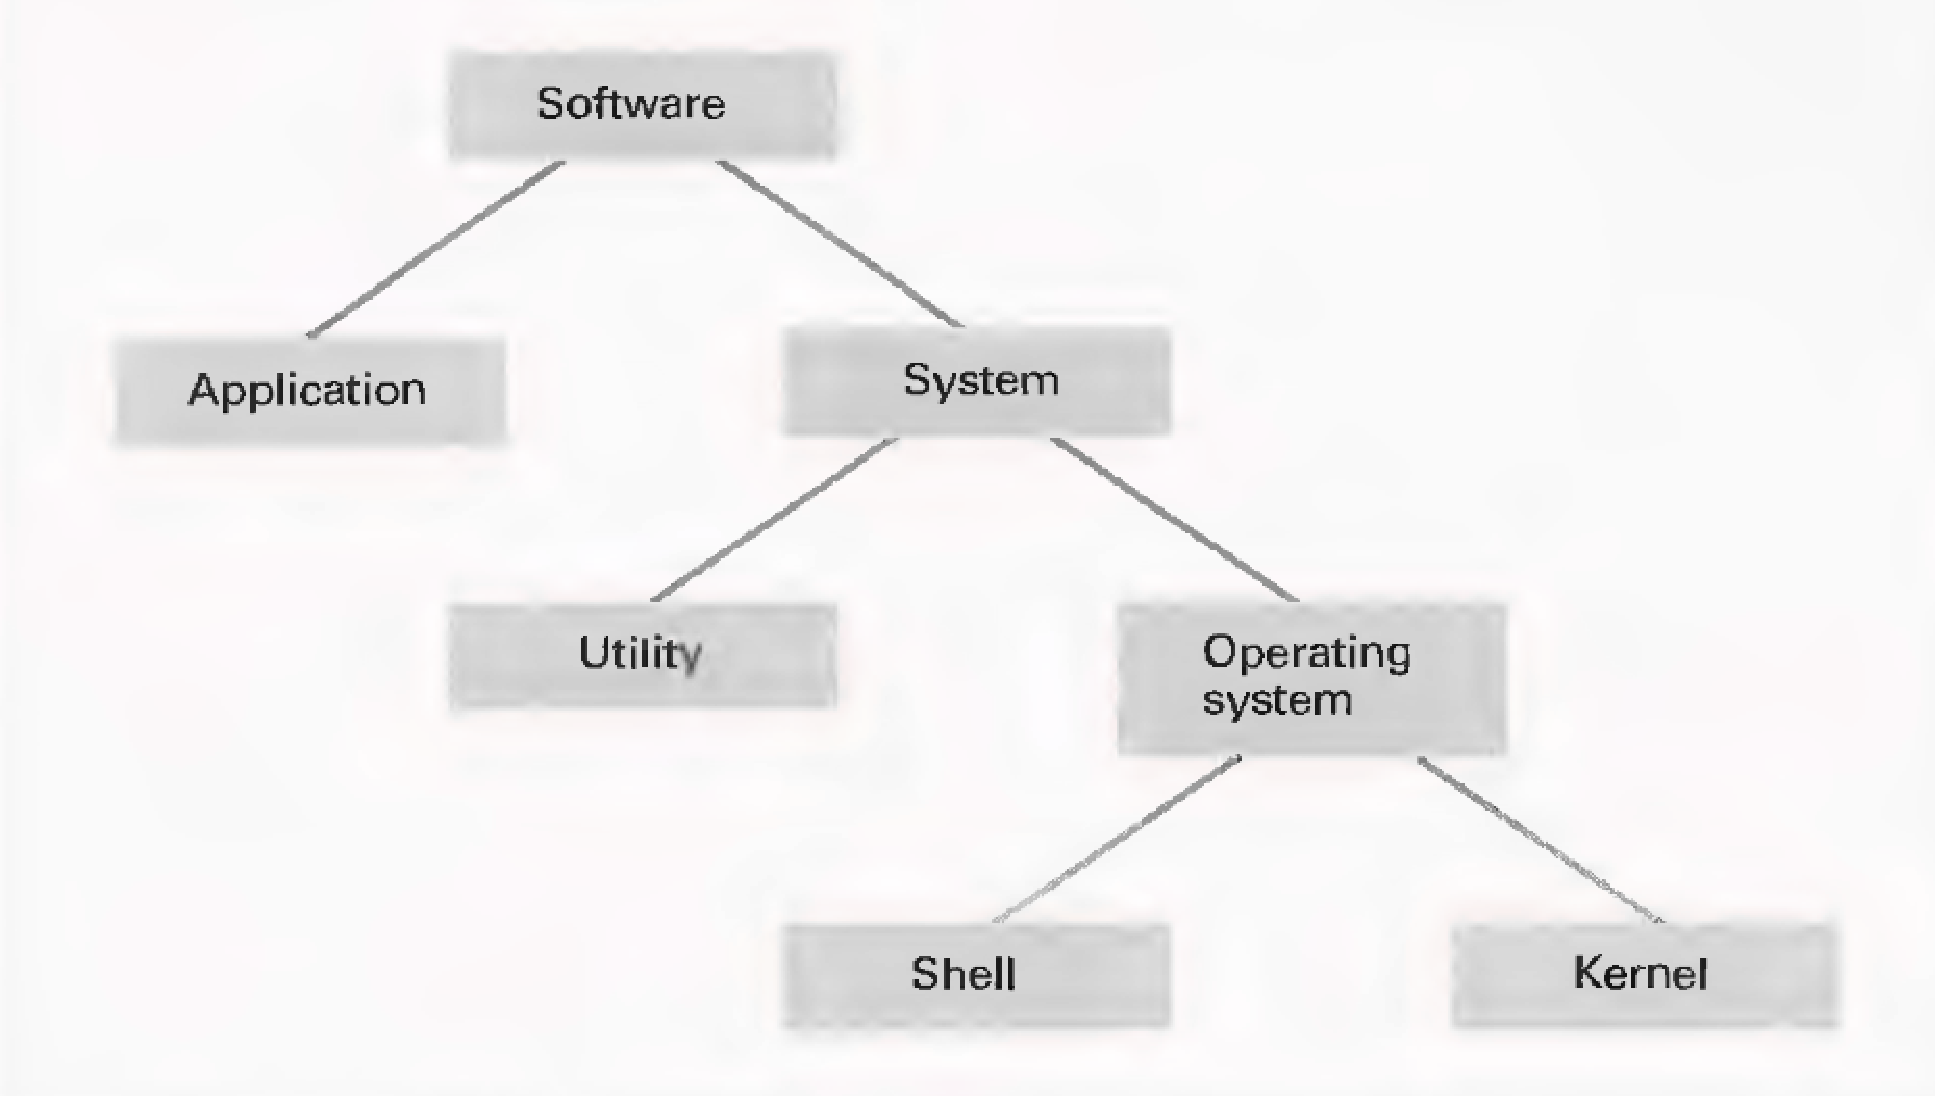
\includegraphics{ch4/fig33.pdf}}
  \caption{Phân loại phần mềm}
  \label{fig:fig3.3}
\end{figure}

Ngược lại với phần mềm ứng dụng là phần mềm hệ thống nhằm thực hiện các nhiệm vụ chung của
các hệ thống máy tính. Theo một nghĩa nào đó, phần mềm hệ thống cung cấp cơ sở hạ tầng cho
các phần mềm ứng dụng. Ta có thể ví nó với cơ sở hạ tầng của một quốc gia (chính
phủ, đường đi lại, các nghành phục vụ, viện tài chính,...) cung cấp cơ sở cho người dân
dựa vào sống theo cách của họ.

Bên trong các lớp các phần mềm hệ thống ta lại chia thành hai phạm trù: một là bản thân hệ
điều hành và hai là những phần mềm khác bao gồm các đơn vị phần mềm tập hợp lại dưới dạng
\textbf{phần mềm công cụ}. Phần lớn phần mềm công cụ cài đặt các chương trình nhằm thực
hiện các hoạt động cơ bản của máy tính nhưng không có sẵn trong hệ điều hành. Theo một
nghĩa nào đó, phần mềm công cụ bao gồm các đơn vị phần mềm giúp mở rộng (cũng có thể để
tuỳ biến) khả năng của hệ điều hành. Ví dụ, chức năng format một đĩa từ hoặc sao chép một
files từ đĩa từ vào đĩa CD thường không được cài đặt bởi hệ điều hành nhưng nó được cung
cấp bởi phần mềm công cụ. Những ví dụ khác của phần mềm công cụ là phần mềm nén và giải
nén dữ liệu, phần mềm để trình diễn đa phương tiện, và phần mềm để thực hiện truyền thông
trong mạng.

Sử dụng các phần mềm công cụ cho phép phần mềm hệ thống có thể tuỳ biến dễ dàng hơn so với
việc đặt chúng có sẵn ngay trong hệ điều hành. Thật vậy, thông thường các công ty hoặc cá
nhân phải thay đổi, hoặc thêm, các phần mềm công cụ vào hệ điều hành trong máy của họ.

Không may mắn, việc phân biệt giữa phần mềm ứng dụng và phần mềm công cụ là không rõ
ràng. Theo quan điểm của chúng tôi, sự khác biệt là gói phần mềm này có là một phần trong
cơ sở hạ tầng phần mềm của máy hay không. Bởi vậy một ứng dụng mới có thể thuộc nhánh công
cụ nếu nó trở thành một công cụ cơ bản. Khi vẫn còn là dự án nghiên cứu, phần mềm để
truyền thông trên Internet đã được xem là phần mềm ứng dụng; ngày nay phần mềm kiểu này là
cơ bản cho hầu hết việc sử dụng PC và bởi vậy nó được phân loại là phần mềm công cụ.



Sự phân biệt giữa phần mềm công cụ và hệ điều hành cũng không rõ ràng. Ví dụ, luật chống
độc quyền ở Mỹ và Châu Âu đã đặt ra câu hỏi liên quan đến phần mềm như trình duyệt web
Internet Explorer và Media Player là một thành phần của hệ điều hành của Microsoft hay chỉ
là phần mềm công cụ mà Microsoft đã cố tình cho vào hệ điều hành nhằm mục đích cạnh tranh.


\subsection*{Các thành phần của một hệ điều hành}

Ta sẽ chú tâm vào thành phần bên trong một hệ điều hành. Để có thể thực hiện các hoạt động
được yêu cầu bởi những người dùng, hệ điều hành phải có khả năng giao tiếp. Thành phần của
một hệ điều hành thực hiện việc giao tiếp này thường được gọi là \textbf{shell}. Các shell
hiện đại thực hiện nhiệm vụ này thường theo hướng \textbf{giao diện đồ hoạ với người dùng
  (GUI)} trong đó các đối tượng cần thao tác như các file và chương trình, được biểu diễn
bằng các biểu tượng trên màn hình. Các hệ thống này cho phép hiểu lệnh của người dùng
thông qua việc trỏ tới các biểu tượng này. Việc này thường được thực hiện nhờ một thiết bị
cầm tay được gọi là chuột. Các shell cũ hơn thường giao tiếp với người dùng qua thông điệp
dạng văn bản sử dụng bàn phím và màn hình.



Mặc dù shell của hệ điều hành đóng vai trò quan trọng trong việc thiết lập các chức năng
của máy, các shell này đơn thuần chỉ là giao diện giữa người dùng và nhân (trái tim) của
hệ điều hành (Hình \ref{fig:fig3.4}). Ta phân biệt giữa shell và phần bên trong của hệ
điều hành như thế này bởi vì một số hệ điều hành cho phép người dùng lựa chọn các shell
khác nhau để có một giao diện phù hợp với từng đối tượng người dùng cụ thể. Ví dụ, người
dùng hệ điều hành UNIX có thể lựa chọn một trong nhiều shell như Bourne shell, C shell, và
Korn shell. Hơn nữa, những phiên bản trước của hệ điều hành Microsoft Windows về mặt cơ
bản đã được xây dựng nhằm thay thế các shell dựa trên văn bản đang sử dụng (trên hệ điều
hành MS-DOS) bằng một shell kiểu giao diện đồ hoạ, tuy nhiên khung của nó vẫn là MS-DOS.

\begin{figure}[tb]
  \centering \scalebox{0.4}{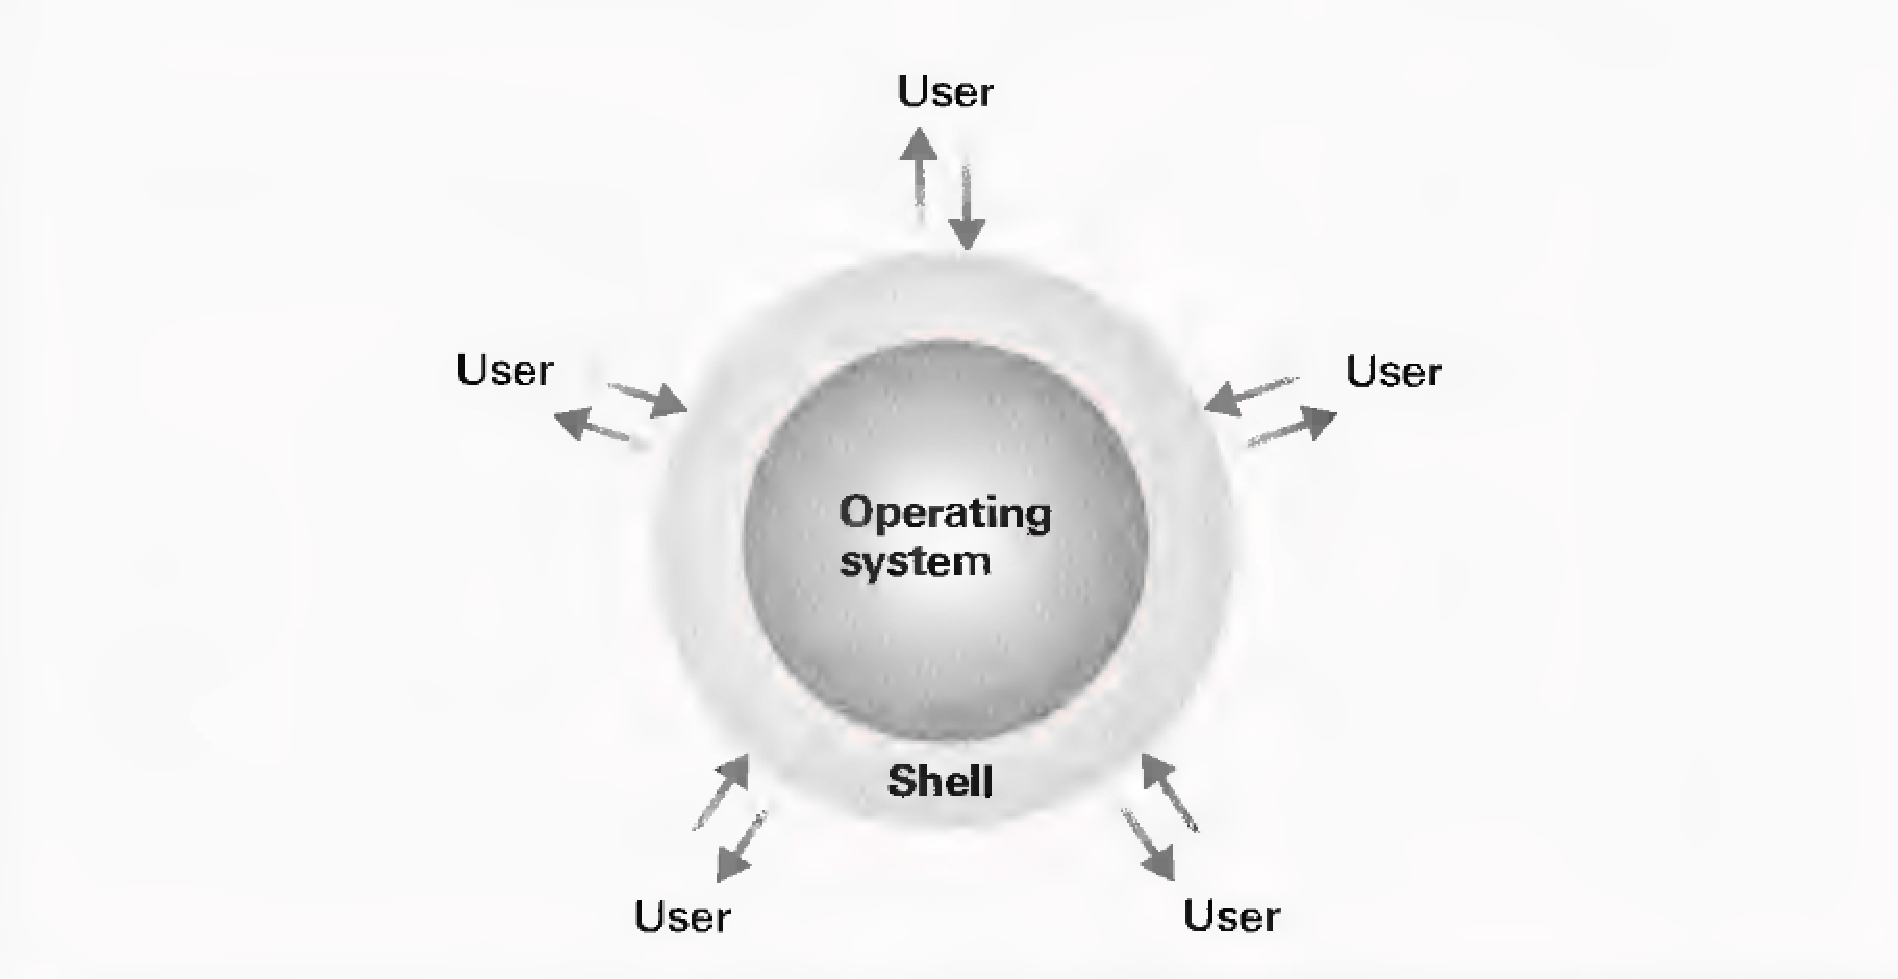
\includegraphics{ch4/fig34.pdf}}
  \caption{Shell như một giao diện giữa người dùng và hệ điều hành}
  \label{fig:fig3.4}
\end{figure}

Một thành phần quan trọng bên trong các shell đồ hoạ của ngày nay là \textbf{chương trình
  quản lý cửa sổ}, với các khối được cấp phát của không gian màn hình, được gọi là cửa sổ,
và mỗi các ứng dụng được gắn với mỗi cửa sổ. Khi một ứng dụng muốn hiện một thứ gì đó ra
màn hình, nó thông báo với trình quản lý cửa sổ, và trình quản lý cửa sổ sẽ đặt các hình
ảnh mong đợi vào trong cửa sổ gắn với ứng dụng. Từ đó, mỗi khi một nút chuột được nhấn,
chính trình quản lý cửa sổ sẽ tính toán vị trí của chuột trên màn hình và gọi ứng dựng
thích hợp tương ứng với thao tác của chuột.

Ngược lại với shell của hệ điều hành, phần bên trong của hệ điều hành được gọi là
\textbf{nhân} (kernel). Một nhân của hệ điều hành chứa các thành phần phần mềm thực hiện
các chức năng rất cơ bản yêu cầu bởi hệ thống máy tính. Một ví dụ là \textbf{trình quản lý
  file}, công việc của nó là phối hợp làm dễ dàng việc sử dụng thiết bị lưu trữ khối của
máy. Chính xác hơn, trình quản lý file chứa các bản ghi của mọi file nằm trong thiết bị
lưu trữ khối, gồm cả vị trí mỗi file được đặt, người dùng nào được phép truy cập vào file
nào, và bộ phận nào của lưu trữ khối sẵn sàng dành cho các file mới, hoặc mở rộng các file
đã tồn tại. Các bản ghi này được giữ ở một nơi lưu trữ trung gian chứa các file liên quan
sao cho mỗi thời điểm nơi trung gian được đặt trực tuyến, trình quản lý file có thể tìm
thấy chúng và biết có gì được lưu trữ ở phần trung gian này.

Để thích hợp với người dùng máy, hầu hết các trình quản lý file cho phép các file được
nhóm lại dưới dạng \textbf{thư mục} (directory hoặc folder). Cách tiếp cận này cho phép
người dùng tổ chức các file của anh hay chị ta theo mục đích bằng cách đặt các file có
liên quan trong cùng một thư mục. Hơn nữa, bằng cách cho phép các thư mục chứa các thư mục
khác, được gọi là thư mục con, một tổ chức theo kiểu phân cấp có thể được xây dựng. Ví dụ,
một người dùng tạo ra một thư mục gọi là \texttt{MyRecords} có chứa các thư mục con là
\texttt{FinancialRecord}, \texttt{MedicalRecords} và \texttt{HouseHoldRecord}. Bên trong
mỗi thư mục con có thể có các file ở một phạm trù đặc biệt (Người dùng hệ điều hành
Windows có thể hỏi trình quản lý file để hiện tập các thư mục hiện hành bằng cách thực
hiện chương trình Windows Explorer).

Một đường đi tới một thư mục bên trong các thư mục được gọi là \textbf{đường dẫn thư
  mục}. Đường dẫn thường được biểu diễn bằng cách liệt kê các thư mục dọc theo đường đi
ngăn cách bởi dấu gạch chéo. Ví dụ,  \texttt{animals/prehistoric/dinosaurs} để biểu
diễn dẫn bắt đầu từ thư mục có tên là \texttt{animals}, qua thư mục con có tên là
\texttt{prehistoric}, và kết thúc trong thư mục con \texttt{dinosaurs}. (Đối với người
dùng Windows, dấu gạch xuôi được thay bằng các dấu gạch ngược lại, ví dụ đường dẫn ở trên
được thay bằng \texttt{animals$\backslash$prehistoric$\backslash$dinosaurs}).

Mọi sự truy cập vào một file bởi một phần mềm khác phải được sự đồng ý của trình quản lý
file theo một thủ tục. Thủ tục bắt đầu bằng cách yêu cầu trình quản lý file kiểm tra quyền
truy cập tới file qua thủ tục mở file. Nếu trình quản lý file đồng ý với yêu cầu truy cập,
nó cung cấp thông tin cần để tìm và thao tác file. Thông tin này được lưu trữ trong một
vùng nhớ được gọi là \textbf{bộ mô tả file} (file descriptor). Phần mềm cần truy cập sẽ
tham khảo các thông tin trong bộ mô tả file này để thực hiện các thao tác nó mong muốn.

Các thành phần khác của nhân (kernel) hệ điều hành bao gồm một tập các \textbf{bộ điều
  khiển thiết bị}, là đơn vị phần mềm chịu trách nhiệm giao tiếp với các bộ điều khiển
(hoặc đôi khi, giao tiếp trực tiếp với thiết bị ngoại vi) để thực hiện các thao tác trên
các thiết bị ngoại vi gắn với máy. Mỗi thiết bị được thiết kế duy nhất cho một kiểu thiết
bị đặc biệt (như máy in, bộ điều khiển đĩa, hoặc màn hình). Nó có trách nhiệm dịch các yêu
cầu chung thành các bước kỹ thuật hơn được yêu cầu bởi thiết bị được gán với bộ điều
khiển. Ví dụ, một bộ điều khiển thiết bị máy in chứa các phần mềm đọc và giải mã các từ mô
tả trạng thái của máy in và các phương pháp giao tiếp kiểu bắt tay khác. Bởi vậy, các
thành phần phần mềm khác không giải quyết được về mặt kỹ thuật cho vấn đề in file. Thật
vậy, các thành phần khác có thể đơn thuần là dựa vào phần mềm điều khiển thiết bị để in
file, còn làm chi tiết thế nào nó để lại cho bộ điều khiển thiết bị. Bằng cách này, việc
thiết kế của các đơn vị phần mềm khác nhau không bị phụ thuộc vào đặc trưng của thiết bị
cụ thể. Kết quả là ta có thể tuỳ biến hệ điều hành cho các thiết bị ngoại vi đặc biệt đơn
thuần bằng cách cài gắn thêm trình điều khiển thiết bị thích hợp.

Một thành phần khác của nhân hệ điều hành là \textbf{quản lý bộ nhớ}, nó chịu trách nhiệm
điều phối việc sử dụng bộ nhớ chính. Trong môi trường đơn nhiệm (máy chỉ thực hiện một
nhiệm vụ tại một thời điểm), nhiệm vụ kiểu này là rất đơn giản. Ở đây, chương trình thực
hiện nhiệm vụ hiện hành đã được đặt trong bộ nhớ, sau khi nó thực hiện xong, bộ nhớ sẽ
được thay thế bởi chương trình thực hiện nhiệm vụ tiếp theo. Tuy nhiên, trong môi trường
đa người dùng hay đa nhiệm, ở đó máy tính phải đáp ứng nhiều yêu cầu tại cùng một thời
điểm, thì việc quản lý bộ nhớ là rất khó khăn. Trong các trường hợp này, nhiều chương
trình và khối dữ liệu phải đồng thời nằm trong bộ nhớ. Bởi thế, trình quản lý bộ nhớ phải
tìm và gán không gian bộ nhớ cho các yêu cầu này và đảm bảo rằng các hoạt động của mỗi
chương trình bị hạn chế trong không gian được cấp phát. Hơn nữa, bởi yêu cầu các hoạt động
khác nhau đến và đi liên tục, trình quản lý bộ nhớ phải nắm bắt được các vùng nhớ nào
không bị còn bận nữa.

Nhiệm vụ của trình quản lý bộ nhớ phức tạp hơn khi tổng số không gian bộ nhớ yêu cầu lớn
hơn so với không gian thực sự có trong máy tính. Trong trường hợp này trình quản lý bộ nhớ
có thể tạo ra cảm giác có không gian lưu trữ thêm bằng cách chuyển chương trình và dữ liệu
qua lại giữa bộ nhớ chính và phần lưu trữ khối (một kỹ thuật gọi là \textbf{phân
  trang}). Giả sử rằng, yêu cầu bộ nhớ chính là $1024$MB nhưng máy tính chỉ có~$512$MB. Để
tạo ra cảm giác có không gian lưu trữ lớn hơn, trình quản lý bộ nhớ dành~$1024$MB không
gian lưu trữ trên đĩa từ để lưu trữ các dãy bít có thể lưu trữ trên bộ nhớ chính nếu bộ
nhớ chính có khả năng thực sự là $1024$MB. Các dữ liệu này được chia thành các khối bằng
nhau được gọi là \textbf{các trang}, kích thuớc các trang này thường chỉ vài KB. Trình
quản lý bộ nhớ điều khiển các trang này tráo đổi giữa bộ nhớ chính và bộ nhớ thứ cấp sao
cho các trang hiện tại cần sẽ nằm trong $512$MB của bộ nhớ chính. Vậy máy tính có thể xử
lý giống như nó có $1024$MB bộ nhớ chính. Không gian bộ nhớ ``tưởng tượng'' này được tạo
bởi cách phân trang được gọi là \textbf{bộ nhớ ảo}.

Nhân hệ điều hành còn có thêm hai thành phần nữa là \textbf{bộ lập lịch} (scheduler) và
\textbf{bộ điều phối} (dispacher). Trong hệ thống chia sẻ thời gian thực, bộ lập lịch xác
định hoạt động nào được thực hiện và bộ điều phối điều khiển việc cấp phát thời gian bộ xử
lý cho các hoạt động này. Ta sẽ nghiên cứu chi tiết hai thành phần này trong mục sau.

\subsection*{Quá trình khởi động máy}
Ta đã thấy rằng hệ điều hành cung cấp cơ sở hạ tầng phần mềm cần thiết cho các đơn
vị phần mềm khác, nhưng ta chưa biết bản thân hệ điều hành bắt đầu như thế nào. Đây
chính là quá trình \textbf{khởi động}, quá trình này được thực hiện mỗi khi máy tính được
bật. Nó là thủ tục nạp hệ điều hành từ thiết bị lưu trữ thứ cấp vào trong bộ nhớ chính
(luôn là rỗng khi máy bật). Để hiểu quá trình khởi động và sự cần thiết của quá trình này,
ta bắt đầu bằng cách xem xét cấu trúc của CPU.

Một CPU được thiết kế có bộ đếm chương trình bắt đầu với một địa chỉ xác định trước mỗi
khi máy bật. Và tại đây, CPU mong đợi tìm thấy một chương trình để thực hiện. Về mặt thiết
kế, ta chỉ cần lưu trữ hệ điều hành bắt đầu tại địa chỉ này. Tuy nhiên, do tính chất của
bộ nhớ chính, dữ liệu bị mất đi sau khi tắt máy nên ta phải tìm cách nạp lại dữ liệu vào
bộ nhớ chính mỗi khi máy tính khởi động lại.

Do vậy, một phần nhỏ của bộ nhớ chính nơi CPU mong muốn tìm thấy chương trình khởi đầu của
nó được xây dựng từ kiểu bộ nhớ bền vững (không bị mất khi tắt máy) gọi là \textbf{bộ nhớ
  chỉ đọc (ROM)}, nội dung của nó không thể bị thay đổi. Tuy vậy, hầu hết bộ nhớ ROM ngày
nay được được xây dựng dựa trên công nghệ bộ nhớ flash (có nghĩa rằng nó không hoàn toàn
là ROM bởi vì nó cho phép ghi lại trong trường hợp cần thiết).



Chương trình được lưu trữ trong ROM gọi là \textbf{chương trình mồi}. Chương trình này
được thực hiện một cách tự động khi máy được bật. Nó có nhiệm vụ điều khiển CPU nạp hệ
điều hành từ vị trí xác định trước trong bộ nhớ thứ cấp (thường là đĩa từ) vào bộ nhớ
chính (xem Hình~\ref{fig:fig3.5}). Khi hệ điều hành đã được đặt trong bộ nhớ chính, chương
trình mồi thực hiện một lệnh nhảy đến vùng nhớ này. Lúc này hệ điều hành tiếp quản và bắt
đầu điều khiển các hoạt động của máy.

\begin{figure}[tb]
  \centering \scalebox{0.35}{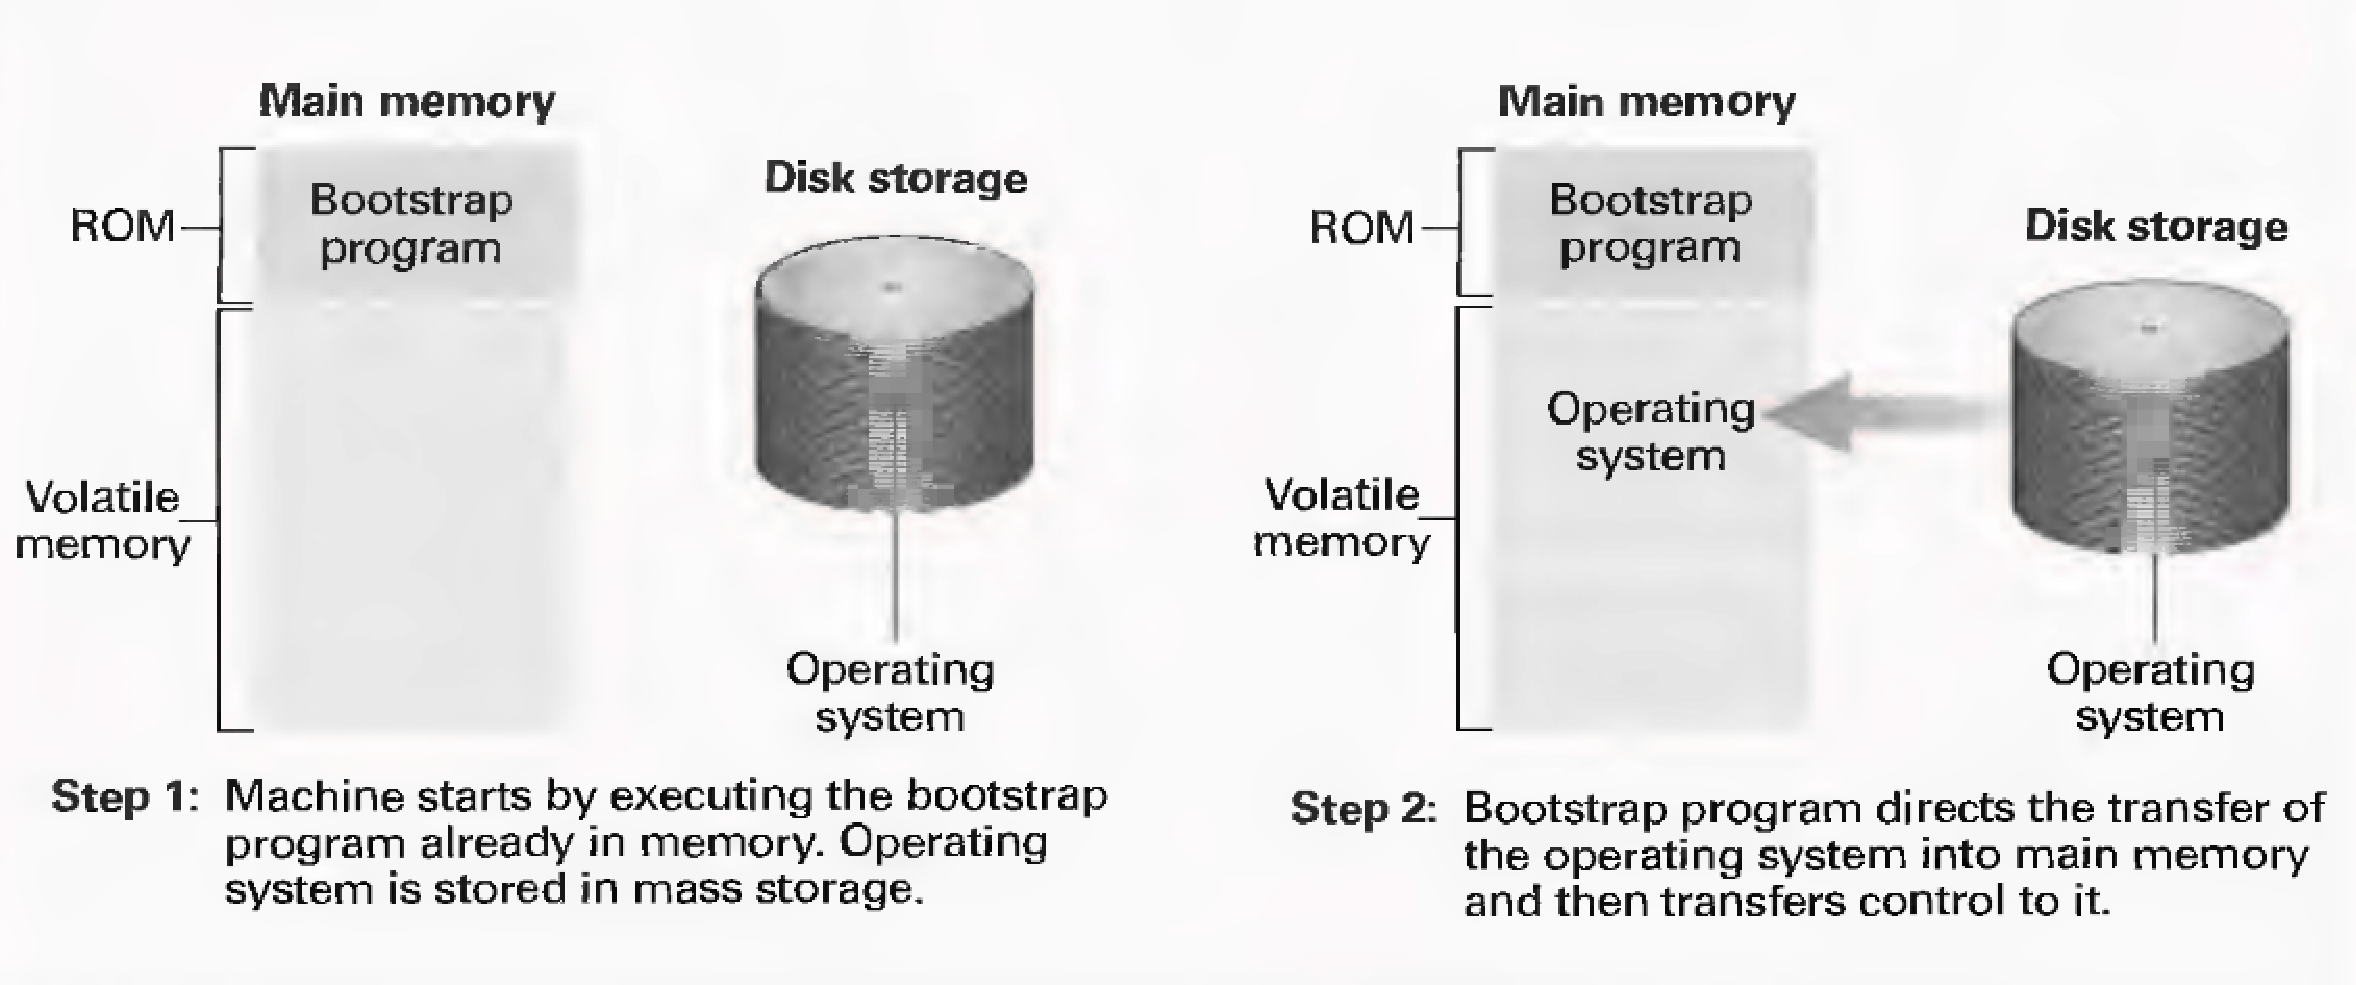
\includegraphics{ch4/fig35.pdf}}
  \caption{Quá trình khởi động}
  \label{fig:fig3.5}
\end{figure}



Một câu hỏi là tại sao không cung cấp đủ ROM để lưu trữ toàn bộ hệ điều hành để tránh phải
nạp từ bộ nhớ thứ cấp. Câu trả lời là do công nghệ hiện tại chưa cho phép dành hẳn một
vùng nhớ lớn của bộ nhớ chính làm vùng lưu trữ bền vững. Tuy nhiên, với sự phát triển
nhanh chóng của công nghệ bộ nhớ, quá trình khởi động mất nhiều bước như thế sẽ sớm trở
nên lạc hâu, và thay vào đó là cách tiếp cận cho phép các phần mềm được lưu trữ lâu bền
trong bộ nhớ.

\subsection*{Câu hỏi \& Bài tập}
\begin{enumerate}
\item Liệt kê các thành phần của một hệ điều hành điển hình và tóm tắt vai trò của mỗi
  thành phần trong một câu.

\item Chỉ ra sự khác nhau giữa phần mềm ứng dụng và phần mềm công cụ.

\item Bộ nhớ ảo là gì?

\item Tóm tắt quá trình khởi động máy.
\end{enumerate}

\section{Điều phối các hoạt động của máy}

Trong phần này ta xem xét cách một hệ điều hành điều phối việc thực hiện phần mềm ứng
dụng, phần mềm công cụ, và bản thân các đơn vị bên trong hệ điều hành. Ta bắt đầu với khái
niệm tiến trình.

\subsection*{Khái niệm tiến trình}
Một trong những khái niệm cơ bản nhất của hệ điều hành hiện đại là phân biệt giữa một
chương trình và hoạt động thực hiện chương trình. Chương trình là một tập tĩnh các chỉ
thị, trong khi đó hoạt động thực hiện chương trình là động, và thay đổi theo thời gian khi
chương trình chạy. Hoạt động này được gọi là \textbf{tiến trình}. Gắn với một tiến trình
là trạng thái hiện hành của hoạt động, được gọi là \textbf{trạng thái của tiến
  trình}. Trạng thái này bao gồm vị trí hiện tại của chương trình đang thực hiện (giá trị
của bộ đếm chương trình) cũng như các giá trị của các thanh ghi và các ô nhớ gắn với
nó. Nói nôm na, trạng thái tiến trình là một ảnh chụp nhanh (snapshot) của máy tại một
thời điểm cụ thể. Những thời điểm khác nhau trong lúc thực hiện chương trình (tại các thời
điểm khác nhau trong một tiến trình) ta quan sát được các ảnh chụp khác nhau (trạng thái
khác nhau của tiến trình).


Trong một hệ thống chia sẻ thời gian thực, thường có nhiều tiến trình tranh chấp tài
nguyên của máy. Nhiệm vụ của hệ điều hành là phải quản lý các tiến trình này sao cho mỗi
tiến trình có tài nguyên (thiết bị ngoại vi, không gian trong bộ nhớ chính, truy cập các
file, và truy cập vào CPU) nó cần, sao cho các tiến trình độc lập không gây trở ngại lẫn
nhau, và sao cho các tiến trình có thể trao đổi thông tin nếu cần.

\subsection*{Quản lý tiến trình}

Các nhiệm vụ liên quan đến việc điều phối tiến trình được thực hiện bởi bộ lập lịch và bộ
điều phối trong nhân của hệ điều hành. Bộ lập lịch duy trì thông tin về tiến trình có mặt
trong hệ thống, đưa các tiến trình mới vào hàng đợi, loại bỏ các tiến trình đã hoàn thành
ra khỏi hệ thống. Bởi vậy, khi người dùng yêu cầu thực hiện một ứng dụng, chính bộ lập
lịch thêm việc thực hiện ứng dụng vào danh sách các tiến trình hiện thời.

Để lưu vết mọi tiến trình, bộ lập lịch duy trì một khối thông tin trong bộ nhớ chính gọi
là \textbf{bảng các tiến trình}. Mỗi khi có yêu cầu thực hiện một chương trình, bộ lập
lịch thêm một mục mới vào trong bảng tiến trình cho tiến trình này. Mục này chứa các thông
tin như vùng bộ nhớ được gán cho tiến trình (lấy từ chương trình quản lý bộ nhớ), độ ưu
tiên của các tiến trình, và trạng thái tiến trình sẵn sàng hay đang đợi. Một tiến trình là
\textbf{sẵn sàng} nếu nó ở trạng thái có thể tiếp tục chạy; nó là \textbf{đợi} nếu hiện
tại nó đang phải đợi cho đến khi một vài sự kiện nào đó bên ngoài xuất hiện, như việc truy
cập đĩa đã hoàn thành, nhấn một phím trên bàn phím, hoặc một thông điệp đến từ tiến trình
khác.



Bộ điều phối tiến trình là thành phần của nhân hệ điều hành chịu trách nhiệm đảm bảo tiến
trình được lập lịch thực sự được thực hiện. Trong hệ thống chia sẻ thời gian thực nhiệm vụ
này được kèm với việc \textbf{chia sẻ thời gian}; có nghĩa rằng, chia thời gian thành
những khoảng ngắn, mỗi khoảng gọi là \textbf{time slide} (thông thường khoảng $50$ mili
giây), và chuyển đổi sự chú ý của CPU tới mỗi tiến trình cho phép mỗi tiến trình thực hiện
trong một time slide (Hình \ref{fig:fig3.6}). Thủ tục chuyển từ tiến trình này sang tiến
trình khác gọi là \textbf{chuyển đổi tiến trình} (process switch) hay \textbf{chuyển ngữ
  cảnh} (context switch).

\begin{figure}[bt]
  \centering \scalebox{0.35}{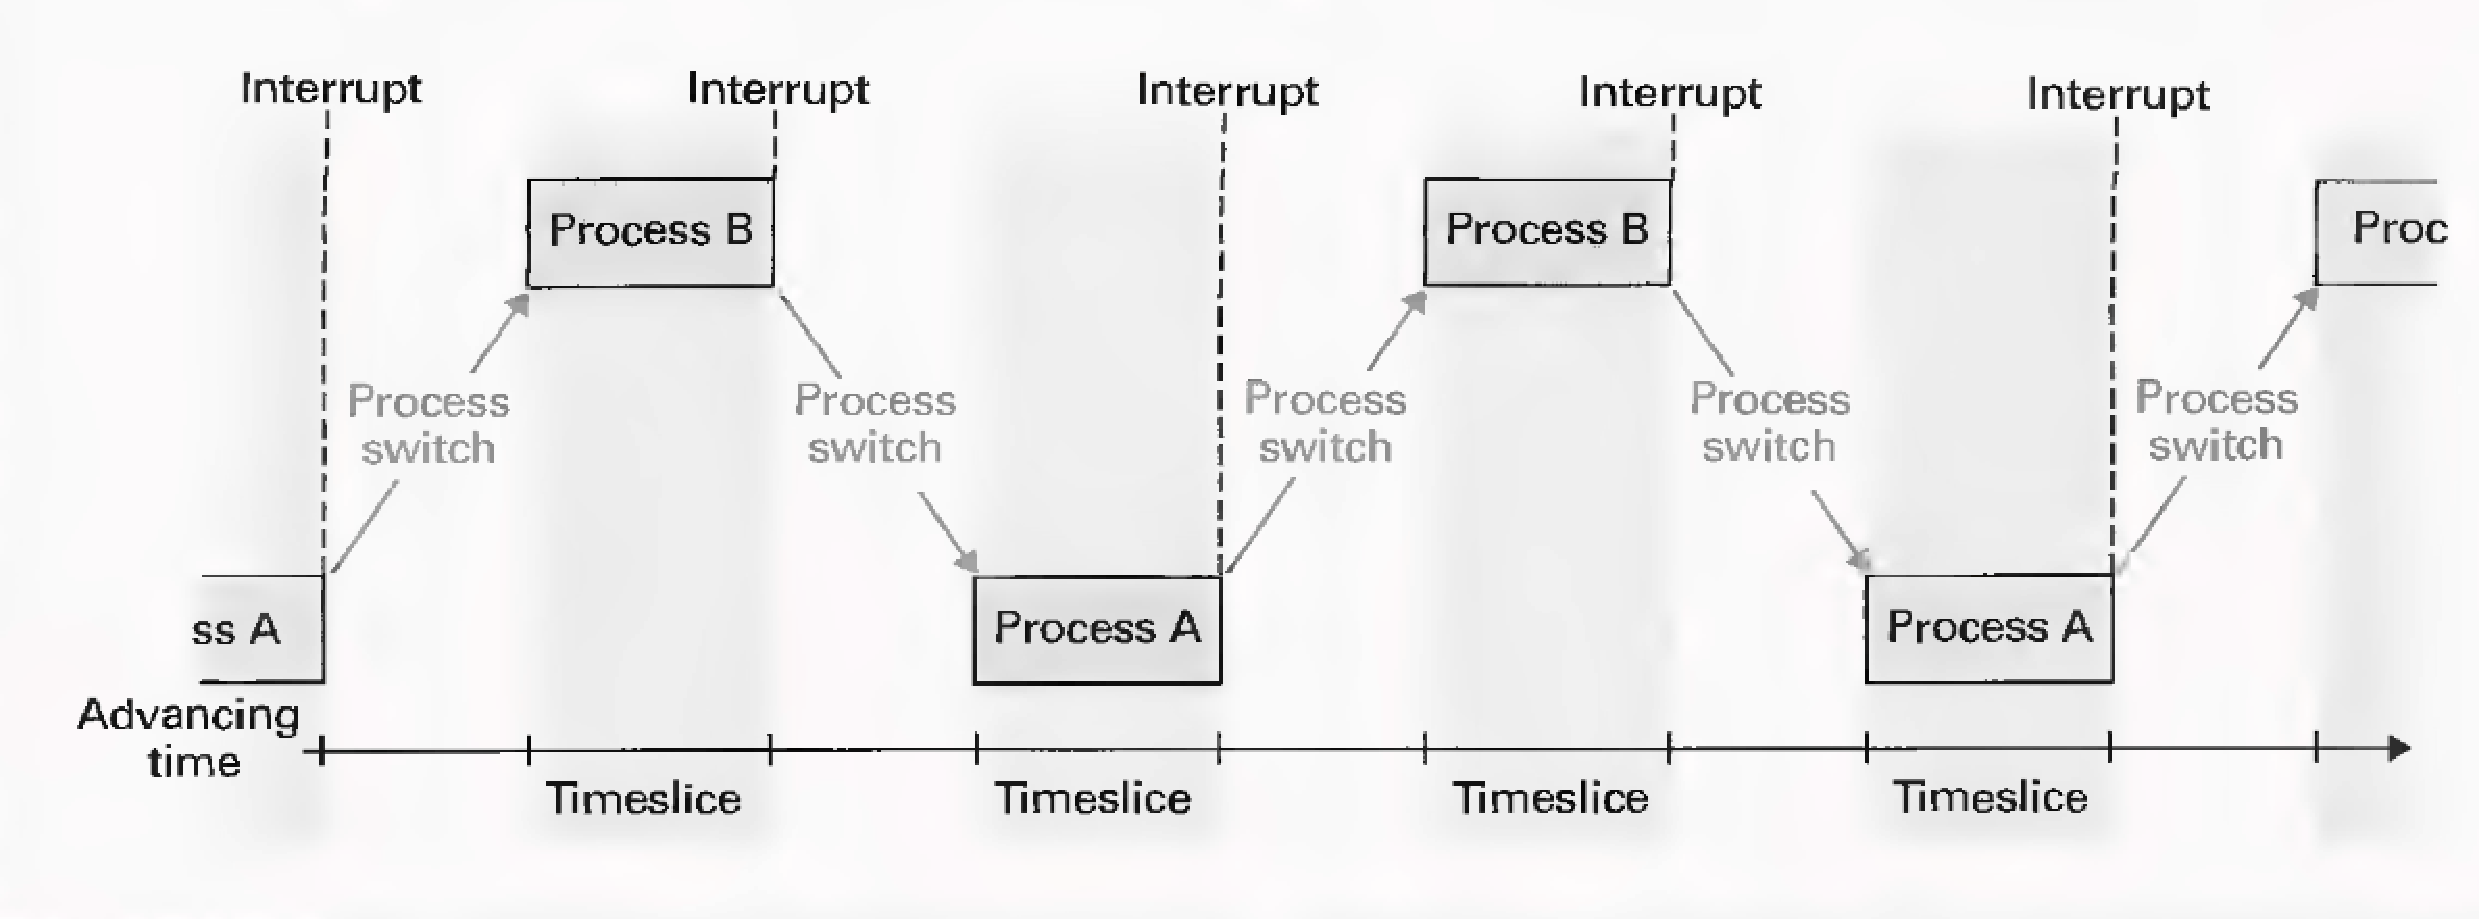
\includegraphics{ch4/fig36.pdf}}
  \caption{Chia sẻ thời gian thực giữa tiến trình $A$ và tiến trình $B$}
  \label{fig:fig3.6}
\end{figure}


Mỗi khi bộ điều phối tiến trình trao time slide cho một tiến trình, nó khởi tạo một mạch
thời gian. Mạch này sẽ sinh ra một tín hiệu gọi là \textbf{ngắt} (interrupt) mỗi khi kết
thúc một time slide. CPU phản hồi lại tín hiệu ngắt này giống như bạn phản ứng khi bị dừng
một công việc. Bạn dừng việc bạn đang làm, ghi nhận lại chỗ công việc bị dừng (để bạn có
thể tiếp tục làm sau), và chuyển sự quan tâm đến đối tượng đòi bạn phải tạm dừng công
việc. Khi CPU nhận một tín hiệu ngắt, nó hoàn thành chu kỳ máy hiện thời của nó, ghi lại
vị trí hiện thời của tiến trình và bắt đầu thực hiện một chương trình, được gọi là
\textbf{trình xử lý ngắt}. Chương trình này được lưu giữ ở một vị trí được xác định trước
trong bộ nhớ chính. Trình xử lý ngắt này là một phần của bộ điều phối, và nó chỉ ra cách
bộ điều phối phải trả lời tín hiệu ngắt.

Bởi vậy, ảnh hưởng của tín hiệu ngắt là để chiếm quyền ưu tiên của tiến trình hiện thời và
chuyển quyền điều khiển lại cho bộ điều phối. Đầu tiên, bộ điều phối cho phép bộ lập lịch
cập nhật bảng các tiến trình (ví dụ, độ ưu tiên của tiến trình vừa hoàn thành time slide
phải thấp hơn độ ưu tiên của các tiến trình khác vừa được đưa vào). Sau đó, bộ điều phối
lựa chọn tiến trình đang sẵn sàng và có độ ưu tiên cao nhất trong bảng các tiến trình,
khởi động lại mạch thời gian, và cho phép tiến trình vừa được lựa chọn bắt đầu time slide
của nó.

Điểm hết sức quan trọng quyết định sự thành công của hệ thống chia sẻ thời gian thực là
khả năng dừng một tiến trình, và sau đó cho phép nó chạy lại. Nếu bạn bị ngắt trong khi
đang đọc sách, khả năng để bạn đọc tiếp sau đó phụ thuộc vào khả năng nhớ vị trí trong
sách cũng như thông tin bạn đã tích luỹ được tính đến thời điểm đó. Nói ngắn gọn, bạn phải
có thể tái tạo lại được môi trường trước thời điểm bị ngắt.

Trong trường hợp của tiến trình, môi trường phải được tái tạo lại là trạng thái của tiến
trình. Nhắc lại rằng trạng thái này bao gồm giá trị của bộ đếm chương trình cũng như nội
dung của các thanh ghi và các ô nhớ thích hợp. Các CPU được thiết kế cho hệ thống chia sẻ
thời gian thực có khả năng kết hợp nhiệm vụ lưu giữ các thông tin này như một phần của
việc phản hồi lại của CPU với tín hiệu ngắt. Các CPU này cũng có các lệnh máy để nạp lại
trạng thái được lưu trữ trước đó. Các đặc điểm này đơn giản hoá nhiệm vụ của bộ điều phối
khi thực hiện chuyển đổi tiến trình và cũng là một ví dụ cho thấy việc thiết kế các CPU
hiện đại bị ảnh hưởng bởi nhu cầu của các hệ điều hành thế nào.

Cuối cùng, ta cũng để ý rằng việc chia sẻ thời gian thực làm tăng hiệu quả của hệ thống về
mặt tổng thể. Điều này đôi khi ngược lại với trực giác của ta vì việc chuyển đổi giữa các
tiến trình yêu cầu bởi hệ thời gian thực làm tốn thời gian của CPU. Tuy nhiên, nếu không
chia sẻ thời gian thực, mỗi tiến trình sẽ phải hoàn thành việc thực hiện trước khi tiến
trình tiếp theo bắt đầu, có nghĩa rằng thời gian tiến trình đợi thiết bị ngoại vi hoàn
thành hoặc đợi yêu cầu từ người sử dụng là bị lãng phí. Còn nếu chia sẻ thời gian thực sẽ
cho phép chuyển CPU đang đợi cho tiến trình khác. Ví dụ, nếu một tiến trình thực hiện một
yêu cầu vào/ra, ví dụ yêu cầu lấy dữ liệu từ đĩa, bộ lập lịch sẽ cập nhật bảng tiến trình
để phản ánh rằng tiến trình này đang đợi một sự kiện bên ngoài. Vậy, bộ điều phối sẽ cắt
time slide của tiến trình này. Sau đó (có thể đến vài nghìn mili giây), khi yêu cầu vào/ra
được hoàn thành, bộ lập lịch sẽ cập nhật bảng tiến trình để chỉ ra rằng tiến trình là sẵn
sàng, và bởi vậy tiến trình này sẽ một lần nữa cạnh tranh để lấy time slides. Tóm lại, một
tiến trình vẫn có thể được thực hiện trong khi yêu cầu vào/ra đang được thực hiện. Bởi
vậy, các nhiệm vụ sẽ được hoàn thành mất ít thời gian hơn so với thực hiện theo cách tuần
tự.

\subsection*{Câu hỏi \& Bài tập}
\begin{enumerate}
\item Tóm tắt sự khác nhau giữa chương trình và tiến trình.

\item Tóm tắt các bước được thực hiện bởi CPU khi một ngắt xuất hiện.

\item Trong hệ thống chia sẻ thời gian, làm thế nào các tiến trình có
  độ ưu tiên cao được phép chạy nhanh hơn so với các tiến trình khác?

\item Nếu mỗi time slide trong hệ thống chia sẻ thời gian là $50$
  milli giây và mỗi việc chuyển đổi ngữ cảnh yêu cầu ít nhất một micro
  giây, có bao nhiêu tiến trình có thể được phục vụ trong một giây?
\label{ex:3.3.4}

\item Nếu mỗi tiến trình sử dụng đầy đủ time slide của nó theo máy ở
  Bài tập \ref{ex:3.3.4}, khoảng thời gian nào của máy thực sự dành
  cho việc thực hiện tiến trình? khoảng thời gian của máy thực sự dành
  cho thực hiện tiến trình là bao nhiêu nếu mỗi tiến trình thực hiện
  một yêu cầu vào/ra chỉ sau một micro giây time slide của nó?
\end{enumerate}







%%% Local Variables: 
%%% mode: latex
%%% TeX-master: "../tindaicuong"
%%% End: 
